\documentclass{lxaiproposal}

\usepackage[english]{babel}

\PassOptionsToPackage{hyphens}{url}\usepackage{hyperref}
\usepackage{times}
\usepackage{array}
\usepackage{color}
\usepackage{epsfig}
\usepackage{pifont}
\usepackage{pifont}
\usepackage{caption}
\usepackage{float}
\usepackage{amsmath}
\usepackage{amssymb}
\usepackage{caption}
\usepackage{amssymb}
\usepackage{pdfpages}
\usepackage{makecell}
\usepackage{svg}
\usepackage{booktabs}
\usepackage{latexsym}
\usepackage{booktabs}
\usepackage{colortbl}
\usepackage{multirow}
\usepackage[compact]{titlesec}
\usepackage{tabularx}
\usepackage{subcaption}
\usepackage{xcolor}

\usepackage[T1]{fontenc}
\usepackage[latin1]{inputenc}

% title config
\titleformat{\section}
  {\Large\bfseries}
  {\thesection}
  {0.5em}
  {}
\titleformat{\subsection}
  {\normalfont\large\bfseries}
  {\thesubsection}
  {0.25em}
  {}

\title{Virtual Node Graph Neural Networks for Hypothetical Metal Organic Framework Inference Tasks\\ \large Summer 2023 PURA Salary Award Proposal}

\author{\coord{Sidharth Baskaran}{}{1}}

\address{\affil{1}{
College of Computing, Georgia Institute of Technology}}

\email{sidharth.baskaran@gatech.edu}

\begin{document}
\maketitle

\section*{Project Overview}

\subsection*{Summary}

In materials science, molecular property prediction has a range of applications, including
energy catalyst optimization and drug discovery. Graph neural networks (GNNs) have proven to be highly effective and scalable for such inference tasks; structurally representing molecules as graphs and scaling to $O(n)$ runtime complexity as opposed to $O(n^3)$ for one of the most popular conventional methods, density-functional theory (DFT). Metal-organic frameworks (MOFs) are porous materials consisting of metal clusters linked by organic components, and pose a challenge for GNNs due to difficulty in expressing pores in graph structures. We propose a model-agnostic method incorporating virtual nodes into molecular graphs for improved expressiveness and performance on MOF prediction tasks that has shown promising results to date. This project is undertaken under mentorship of Dr. Victor Fung (\textit{Georgia Tech CSE}) and in collaboration with Dr. Guojing Cong (\textit{Oak Ridge National Laboratory}).

\subsection*{Message-Passing Graph Neural Networks}

Graph neural networks (GNNs) have become increasingly popular in the materials science space, and can be used on a variety of tasks, including property inference, synthesis prediction, and structure generation\cite{Reiser2022}. In principle, GNNs are able to perform convolutions over arbitrary inputs with standardized feature dimensions, and offer the advantage of working with atomic structures that easily translate to graphs. A graph $G=(v,e,u)$ is represented by a set of nodes $v$, edges $e$, and global properties $u$. Nodes are assigned attributes ${\bf x}\in \mathbb{R}^{n}$ and edges ${\bf e}\in \mathbb{R}^m$. Message-passing (MP) GNNs propagate information between adjacent nodes $v_i,v_j$ across $e_{ij}$, a concept used in modern graph convolutional operators such as in CGCNN (Crystal Graph Convolutional Neural Network)\cite{Xie_2018} which perform complex node attribute update schemes of the form in (\ref{eq:mpupdate}) where for a $k$th update step, $\bigoplus$ is a differentiable, permutation-invariant reduction such as mean, max, sum, and $\gamma,\phi$ are multilayer perceptrons (MLPs).

\begin{equation}
    \mathbf{x}_i^{(k)} = \gamma^{(k)} \left( \mathbf{x}_i^{(k-1)}, \bigoplus_{j \in \mathcal{N}(i)} \, \phi^{(k)}\left(\mathbf{x}_i^{(k-1)}, \mathbf{x}_j^{(k-1)},\mathbf{e}_{j,i}\right) \right)
    \label{eq:mpupdate}
\end{equation}

Each atom in a structure is a node in the graph, and is assigned a vector of node attributes encoding chemical and neighboring properties. Bonds are represented by edges and are assigned vectorial attributes encoding spatial information (\ref{fig:messagep}). Molecular property inference involves scalar-valued predictions given graph inputs. A common pipeline involves a series of convolutional layers followed by a set of fully-connected classification layers to provide a global readout value (\ref{fig:pipeline}). A more in-depth survey can be found at \cite{sanchez-lengeling2021a}.

\begin{figure*}[h]
    \centering
    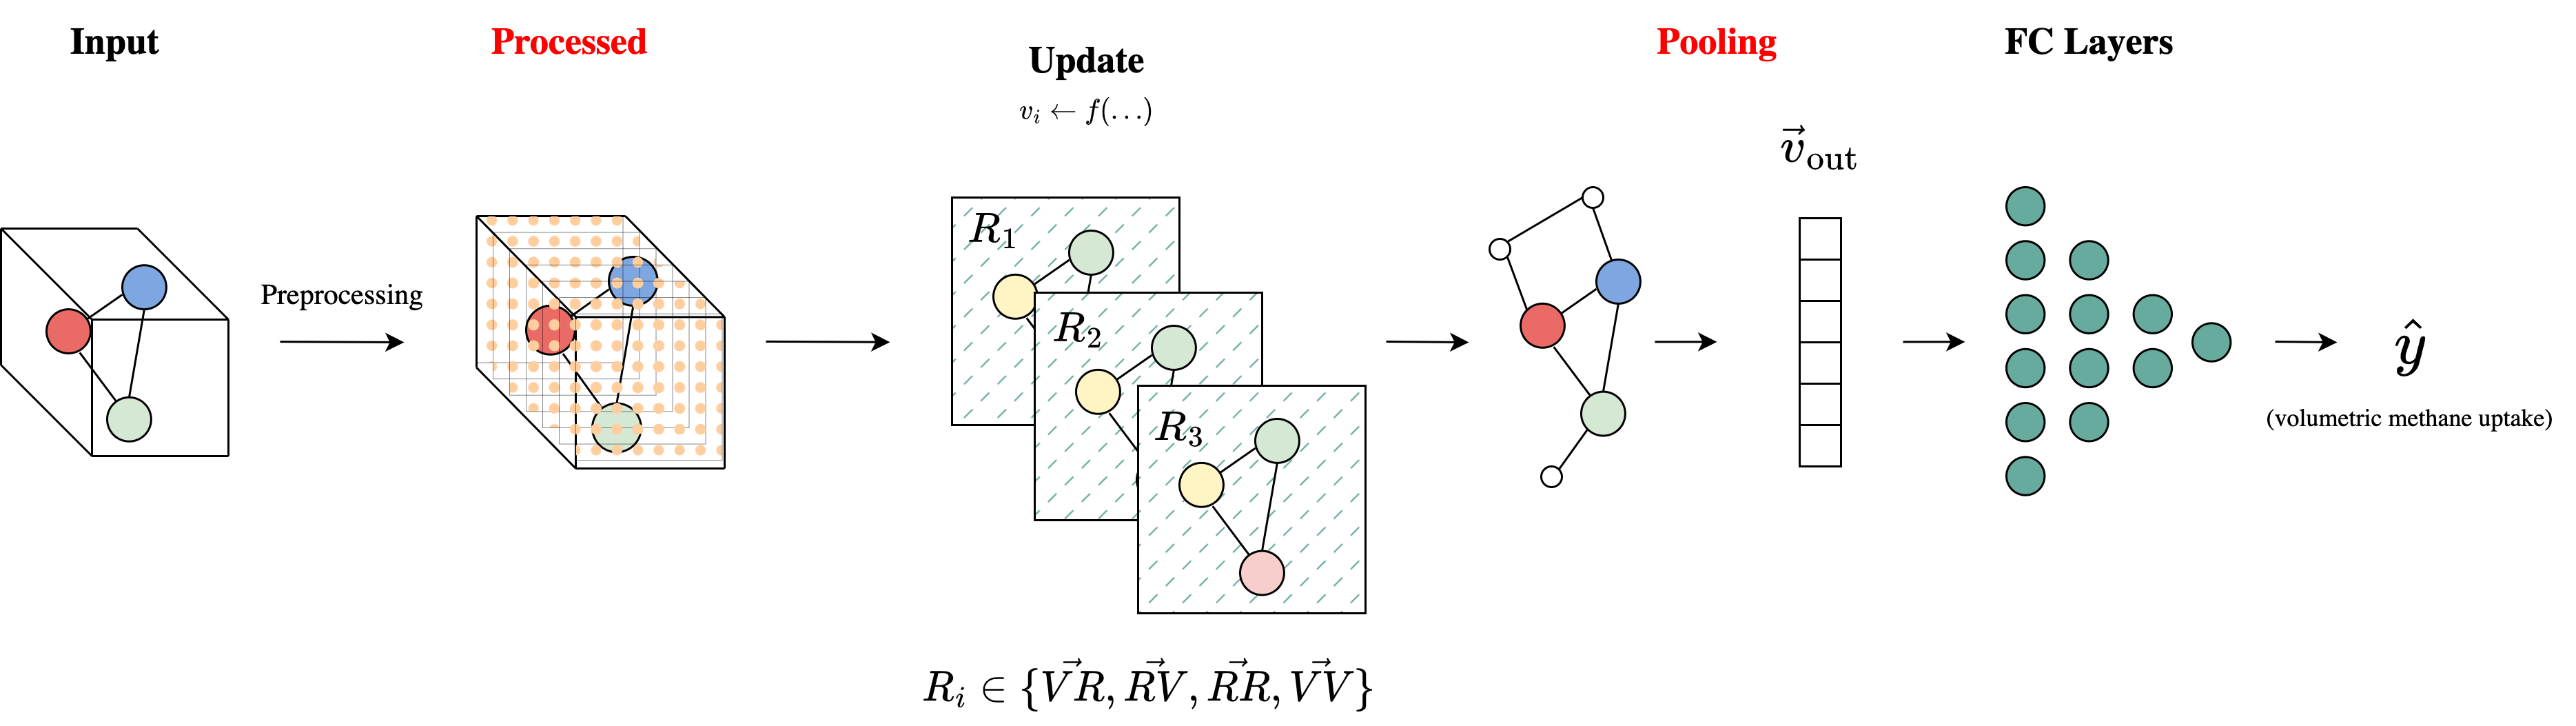
\includegraphics[width=\textwidth]{mdl-vn-pipeline.drawio.png}
    \caption{Volumetric methane uptake inference pipeline with virtual nodes in MatDeepLearn\cite{fung2021benchmarking}}
    \label{fig:pipeline}
\end{figure*}

\begin{figure}
    \centering
    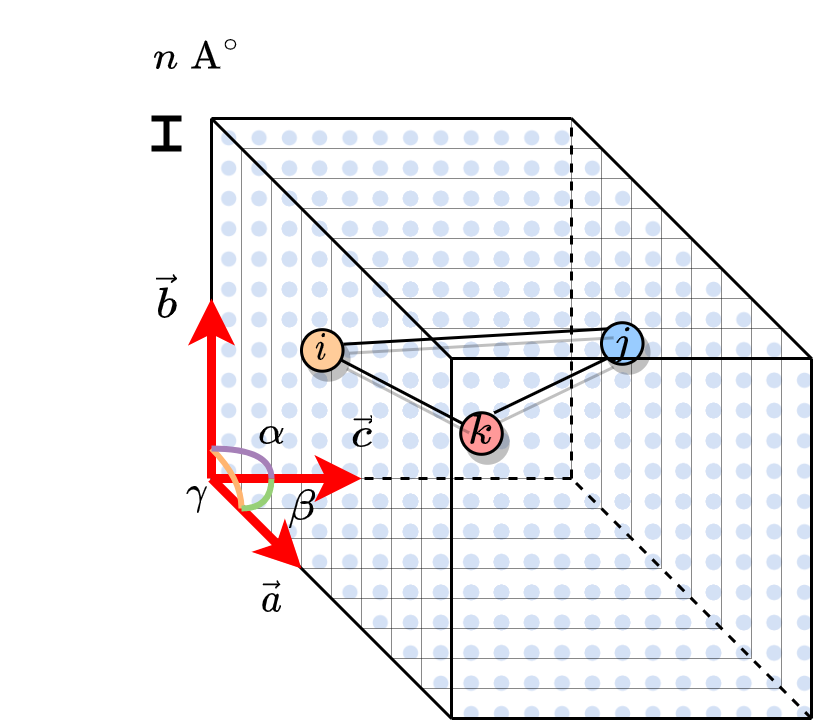
\includegraphics[scale=0.15]{unitcell-vn.drawio.png}
    \caption{Unit cell with virtual node mesh of $n$ A$^\circ$ spacing}
    \label{fig:unitcell}
\end{figure}

\begin{figure*}[h]
    \centering
    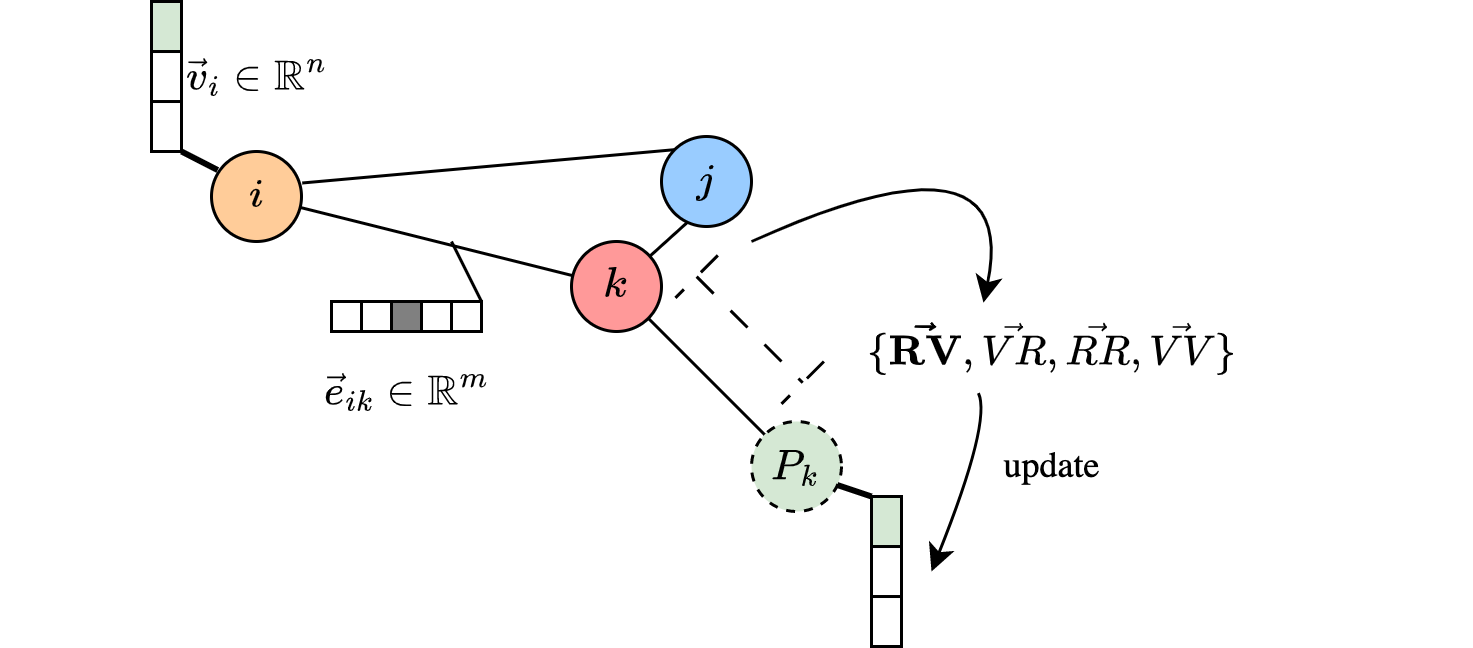
\includegraphics[scale=0.15]{graph-rep-vn.drawio.png}
    \caption{Selective message passing}
    \label{fig:messagep}
\end{figure*}

\subsection*{hMOF Dataset}

Metal-organic frameworks (MOFs) are composed of modular building blocks that form crystal structures, and are of interest due to their porous nature among other properties. The space of  MOFs is large due to their modular structure, which allows for millions of possible structures. The hypothetical metal-organic framework (hMOF) generation procedure generates every possible structure under constraints to produce 137,953 hMOFs, using building blocks of naturally occurring MOFs. The global properties for each structure are surface area, pore volume, pore-size distribution, powder X-ray diffraction pattern, and methane-adsorption capability\cite{wilmer2012large}.

\subsection*{Virtual Nodes for Graph Structures}

Crystal structures are an infinite system GNNs use the graph of the smallest repeating unit (unit cell) as an approximation for the system, described by a set of basis vectors. Virtual nodes are throughout the unit cell parallelepiped to form a controllable mesh (\ref{fig:unitcell}). Each virtual node is described by a node attribute vector and is connected via edges to real and virtual nodes (\ref{fig:messagep}). This approach introduces a set of hyper-parameters (\ref{table:vn-hparam}) in addition to those of the candidate model (i.e. CGCNN).

\begin{table}[h]
        \begin{tabularx}{\linewidth}{p{0.2\linewidth} p{0.05\linewidth} p{0.6\linewidth}}
            \toprule
            \multicolumn{1}{c}{\textbf{Parameter}} & \multicolumn{1}{c}{\textbf{Unit}} & \multicolumn{1}{c}{\textbf{Description}} \\
            \midrule
            Virtual box increment & A$^\circ$ & Spacing between virtual nodes along each dimension of unit cell \\
            MP selectivity & -- & Interaction possibilities at each convolution layer, formally $R\subset I = \{\vec{RV},\vec{RR},\vec{VR},\vec{VV}\}$\\
            Interaction cutoff radius & A$^\circ$ & Cutoff radius for message-passing for each $m\in I$.\\
            Pooling method & -- &  1) Separate pooling on virtual and real nodes, followed by concatenating the results. 2) Given each atomic number, create a separate embedding size $n$ to create a $kn$ size vector for $k$ different atomic numbers.\\
            Pooling scheme & -- & Permutation invariant like sum, mean, min, max.\\
            \bottomrule
        \end{tabularx}
        \caption{Virtual-node-specific hyper-parameters}
        \label{table:vn-hparam}
\end{table}

\section*{Research Plan and Methods}

\subsection*{Preliminary Results}

Without virtual nodes, we use $R=\{\vec{RR}\}$ with an interaction of 5 A$^\circ$.
Baseline tests for virtual nodes were done with $R=\{\vec{RV},\vec{RR}\}$ with interaction cutoff of 5 A$^\circ$, virtual box increment of 3 A$^\circ$, and atomic-number based pooling (\ref{table:vn-hparam}) using mean reduction. The candidate model used was CGCNN, with non-virtual node-specific hyperparameters fixed. A subset of 5000 examples of the hMOF dataset was used in the interest of time, with training, testing, and validation splits of 0.85, 0.15, and 0.05 respectively. Training and validation losses for tests with and without virtual nodes are shown in Figure (\ref{plot:prelim-results}), indicating that the use of virtual nodes provides significant improvement for this inference task.

\begin{figure}[h]
    \centering
    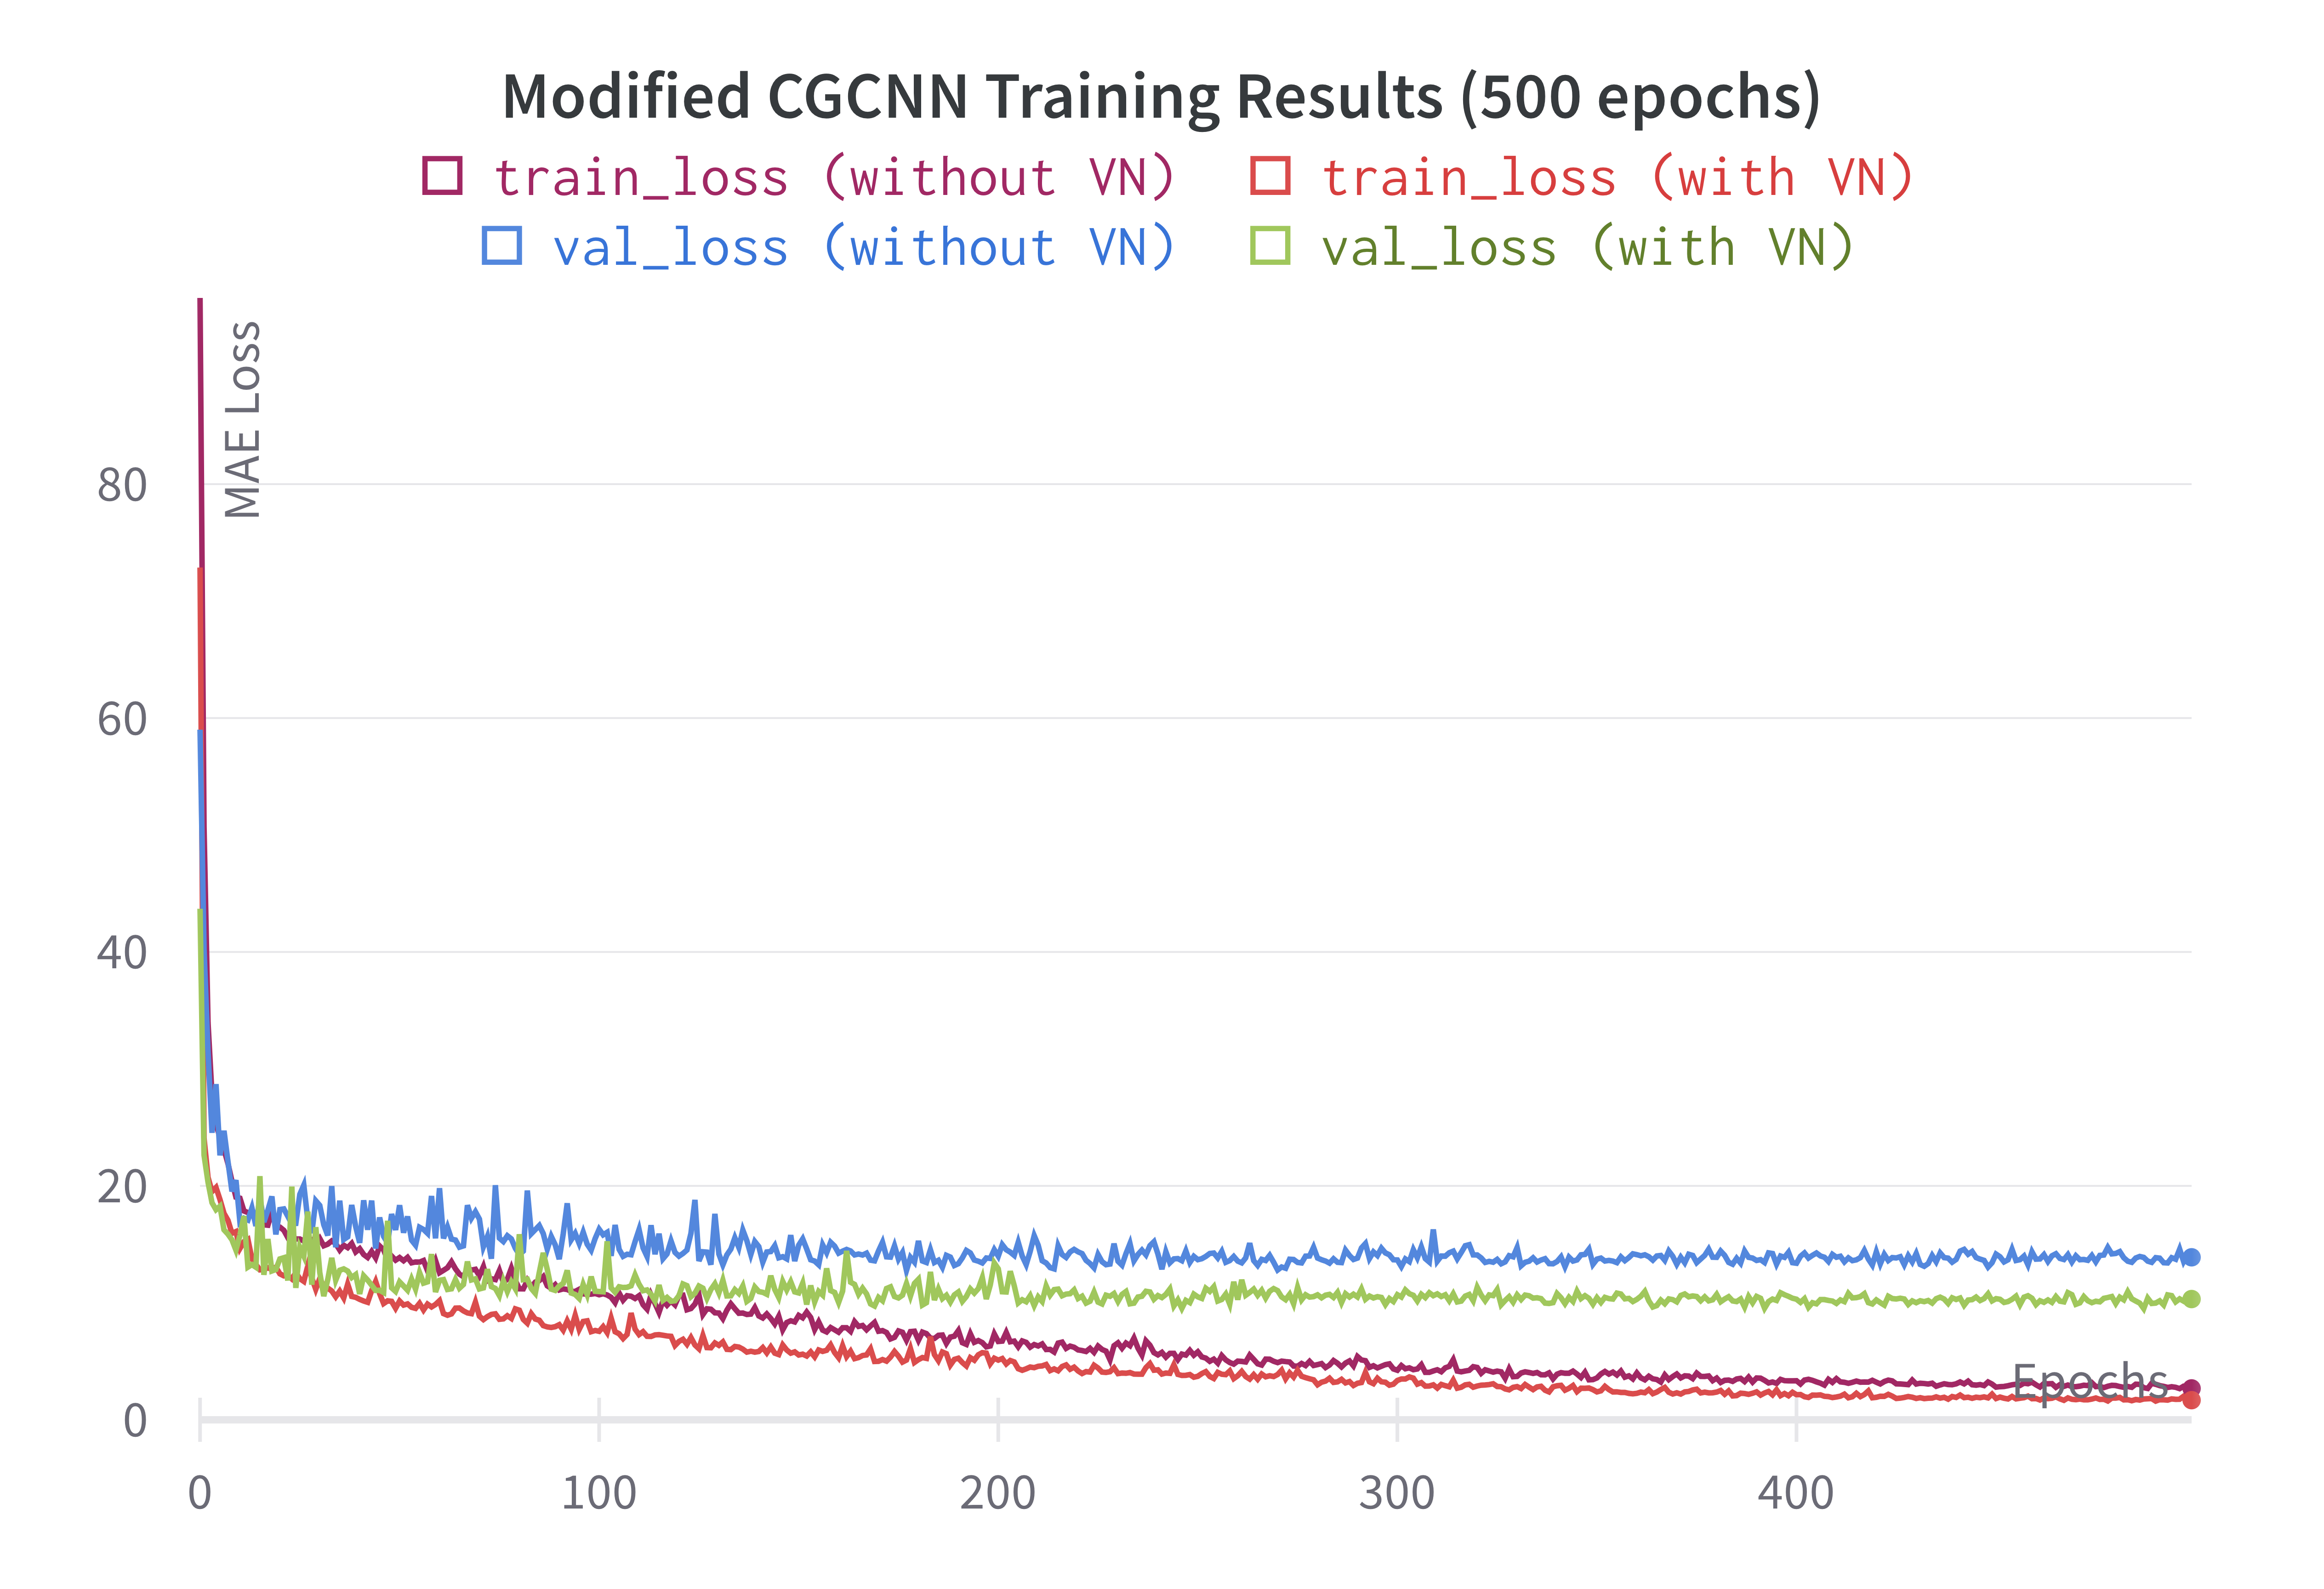
\includegraphics[width=\linewidth]{result-plots-wandb.png}
    \caption{Preliminary results of training on CGCNN model (lower MAE loss is better)}
    \label{plot:prelim-results}
\end{figure}

\subsection*{Hyper-parameter Optimization}

In order to further improve performance from the baseline, our approach will involve virtual node-specific (\ref{table:vn-hparam}) hyper-parameter tuning to identify the most influential parameters.
Specifically, the readout and pooling phase of the model also high potential for improvement through combining different pooling schemes with new custom methods. A current limitation with our readout phase is the high dimensional reduction occurring from the atomic number pooling scheme, which involves a mapping from a $kn$ size feature vector $\vec v_\text{out}$ to a set of fully-connected layers mapping $\approx n\to 1$ (\ref{fig:pipeline}). We are currently working on methods to address this loss of expressiveness. Furthermore, current developments in the GNN space offer model architectures with significant efficiency and performance improvement over CGCNN, providing better options for virtual-node candidates. 

\subsection*{Heterogeneous Graphs}

Heterogeneous graphs provide a way to separate different classes of nodes and edges and learn a separate set of model weights for each class. Treating virtual nodes and real nodes as separate classes allows each class to incorporate a separate set of model weights, improving expressiveness and allowing each class to incorporate a different method of encoding node and edge features. While this increases complexity and memory overhead, approaches such as parallelizing over multiple GPUs and transfer learning are possible solutions.

\subsection*{Methods}

We utilized the pre-processing and training pipeline provided by MatDeepLearn\cite{fung2021benchmarking}, software I actively help develop in collaboration with the Fung Group, to prototype and test our methods. We used either 1 NVIDIA A100 40GB or A40 48GB GPUs to train models on high-performance computing resources provided by National Energy Research Scientific Computing Center's Perlmutter supercomputer, and Georgia Tech's PACE Hive and Phoenix clusters\cite{PACE}. We also utilized PyTorch\cite{pytorch} and PyTorch Geometric for graph learning routines and optimized sparse tensor arithmetic \cite{Fey2019FastGR}. We utilized Weights and Biases\cite{wandb} automated hyper-parameter tuning and experiment tracking.

\section*{Related Work}

Machine learning-based approaches to predict methane-adsorption exist, but do not utilize GNNs, rather creating structural fingerprint vectors encoding spatial and chemical information. Deep neural networks are then used to map these fingerprints to predicted methane-adsorption. \cite{gurnani2021interpretable}. 
Virtual nodes have been used in GNNs for materials property inference, but for different use cases including full phonon\cite{https://doi.org/10.48550/arxiv.2010.09435} and electron density prediction\cite{jorgensen2022equivariant}.

\bibliographystyle{ieee_fullname}
\bibliography{references}

\end{document}